\documentclass[../main.tex]{subfiles}
\begin{document}
In the following chapter a general overview over the ECU structure is given, the focus will be then directed towards the communications protocols between different ECUs and between the ECU and the embedded code that lays in them with an analysis of the AUTOSAR standard. 
\section{ECUs in a modern vehicle}
In the automotive industry there´s been a remarkable evolution over the last few years in which embedded control systems have grown from stand alone control to highly integrated networked control systems \cite{Johansson_vehicleapplications}. The growth require a process of implementing the scalability also in the development process, via efficient communication protocols and standardize software interfaces passing through the control units. 
ECU can be considered as the brain of the modern cars. The ECU uses a closed loop control system that based on the system outputs control the inputs in order to make the engine works.\\
The key to a fast response is a fast computation time. The ECU code need to be optimized to run as fast as possible in order to reposed efficiently to the fast changing engine parameters. 
It´s possible to enumerate the main control units present in most of modern vehicles:
\begin{itemize}
    \item ECU, Engine control module, ensure the correct functionality of everything related to the engine
    \item BCM, Brake control module, control the part related to break and breaking systems, such as ABS.
    \item TCM, Transmission control module, control the transmission.
    \item TCU, Telematic control unit, control the HMI and other user services offered by the vehicle. 
    \item SCM, Suspensions control unit, control suspension, especially with upcoming technology related to active suspension control. 
\end{itemize}


\section{Hardware structure of an ECU}
\begin{figure}[h]
    \centering
    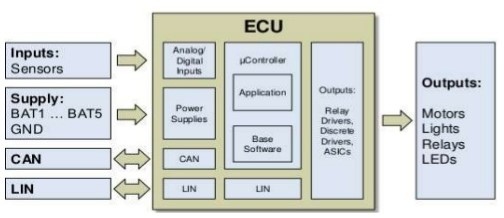
\includegraphics[width=\linewidth]{images_folder/electronic-control-unitecu-6-638.jpg}
    \caption{ECU structure}
    \label{fig:ECUHW}
\end{figure}
The hardware structure of an ECU is composed by complex series of components, to better understand the overall organization, without entering in to much of a engineering detail a block scheme overview is offered by \ref{fig:ECUHW}.\\
It´s possible to easily differentiate between four different parts:
\begin{itemize}
    \item Power supply, handle the power input for the board and for the power components such as the motor driver or other power electronics components needed to drive the controlled parts. 
    \item Inputs, which can be either analog and digital inputs
    \item Communications link, such as CAN and LIN.
    \item Outputs, the output are mainly composed by mechanical components that require electrical actuation in order to perform engine required tasks. Other output that can be found are related to the sharing of information with other ECUs.
    \item MPU, Microprocessor unit and memory, in general Flash and RAM. 
\end{itemize}
\subsection{CAN - Communication protocols in ECU}
The Controll Area Network (CAN) is a serial communication protocol suited for networking sensors, actuators and other node in real-time systems. The CAN specifications define the protocols only for the physical layers and the data link layers. These layers are part of the OSI, Open System Interconnections, an abstraction model for communication protocol. 
\begin{figure}[h]
    \centering
\begin{tikzpicture}[box/.style={on chain,join,draw,minimum width=4cm,minimum height=1cm,
align=center},start chain=going below, node distance=5mm,font=\sffamily,fbox/.style={draw,thick,fill=white}]
  \node[box] (a) {Application layer};
  \node[box] (b) {Presentation layer};
  \node[box] (c) {Session layer};
  \node[box] (d) {Transport layer};
  \node[box] (e) {Network layer};
  \node[box] (f) {Data Link layer};
  \node[box] (g) {Physical layer};
  \node[above=1cm, xshift=1mm] (l) {Application A};
  \begin{scope}[on background layer]
   \node[fbox,fit=(a|-l.north) (g),inner xsep=3mm] (f1){};
  \end{scope}
\end{tikzpicture}
    \caption{OSI}
    \label{fig:ECUstructure}
\end{figure}
The OSI is an abstraction model for the communications protocols. The main layer that are needed to be analyzed are the physical layer and the Data link layer. Just for reference purpose the top upper layer, the application layer defines what to do with the data received in the physical layer.\\
The physical layer is indeed composed by the physical transport media, form cables to the plug and sockets. CAN use a twisted pair in which the differential voltage between the couple is used to represent the bits transmitted. The Data link layer defines the MAC, Media Access Control Methods. In CAN this is set to CSMA/CA or Carrier Sense Multiple Access/ Collision Avoidance. What this complex series of acronyms stand for is that in CAN on the bus a message can be sent only if the bus is free, in case two nodes send a message contemporaneously, then the message with the highest priority win and the node with the low priority message retrieve to a receiver status. 
\section{Autosar standards}

\cleardoublepage
\end{document}
